\documentclass[12pt]{article}
\usepackage{graphicx} % Required for inserting images
\usepackage{blindtext}
\usepackage{titlesec}
\usepackage{relsize}
\usepackage{fancyhdr}
\usepackage{listings}
\usepackage[italian]{babel}
\usepackage{xcolor}
\usepackage{array}
\usepackage{hyperref}
\usepackage[left=3cm,right=3cm, margin=3cm, vmargin=3cm]{geometry} % Imposta i margini laterali a 3 cm
\usepackage[utf8]{inputenc}
\usepackage{tcolorbox} % pacchetto per creare scatole colorate
\definecolor{codegreen}{rgb}{0,0.6,0}
\definecolor{codegray}{rgb}{0.5,0.5,0.5}
\definecolor{codepurple}{rgb}{0.58,0,0.82}
\definecolor{backcolour}{rgb}{0.95,0.95,0.92}
\lstdefinestyle{mystyle}{
    backgroundcolor=\color{backcolour},   
    commentstyle=\color{codegreen},
    keywordstyle=\color{magenta},
    numberstyle=\tiny\color{codegray},
    stringstyle=\color{codepurple},
    basicstyle=\ttfamily\footnotesize,
    breakatwhitespace=false,         
    breaklines=true,                 
    captionpos=b,                    
    keepspaces=true,                 
    numbers=left,                    
    numbersep=5pt,                  
    showspaces=false,                
    showstringspaces=false,
    showtabs=false,                  
    tabsize=2
}
\lstset{style=mystyle}

\begin{document}
\begin{titlepage}
    \begin{center}

        
\includegraphics[width=0.75\textwidth]{Uniroma1.svg.png}
        \par\medskip\noindent \\

        \large{Università "Sapienza" di Roma\\

            Facoltà di Informatica\\

            \textbf{Corso}: Metodologie Di Programmazione}\\

        \vfill

        \textbf {\Huge{Documentazione JPokeBattle}}
        \par\medskip\noindent \\
        \large{\textbf{Author: }Alessia Cassetta}\\

        \large{\textbf{Matricola: }2113909}

        \large{\textbf{Email:} cassetta.2113909@studenti.uniroma1.it}

        \large{\textbf{GitHub:}\href{https://github.com/ajhxia/UNI/tree/main/Primo%20Anno/Metodologie%20di%20Programmazione/Project-JPokeBattle}{Progetto JPokeBattle}}

        \vfill

        \textbf{Anno Accademico 2023/2024}

    \end{center}
\end{titlepage}
\newpage
\tableofcontents
\newpage

\section{Feature Sviluppate}
\begin{itemize}
    \item \textbf{Minimo}
          \begin{itemize}
              \item Implentati 55 pokemon di prima generazione, con le loro mosse base e statistiche.
              \item Assegnati a tutti i Pokémon le due mosse di tipo neutro apprese al livello 1.
              \item Implementare le schermate “start”, battaglia, cambio pokémon, “you win”, e “game over”.
              \item Adottata Java Swing
              \item Far affrontare al giocatore una serie di avversari NPC, fino alla sua prima sconfitta.
          \end{itemize}
    \item \textbf{Tipico}
          \begin{itemize}
              \item Preservare lo stato dei pokémon del giocatore nella serie di lotte.
              \item Implementate tutte le mosse dei Pokémon scelti, rispettando le loro meccaniche di funzionamento dipendenti dai loro tipi, ma ignorando i cambiamenti di stato come avvelenamento, stordimento, etc.
              \item Implementare una schermata leaderboard che mantenga i 10 record migliori.
          \end{itemize}
    \item \textbf{Extra}
          \begin{itemize}
              \item Set crescita:
                    \begin{itemize}
                        \item Implementare punti individuali e punti allenamento che migliorino le capacità dei pokémon sulla base delle vittorie, aggregandoli appropriatamente.
                        \item Implementare i meccanismi di passaggio di livello ed evoluzione dei Pokémon, incluso l’apprendimento di nuove mosse a determinati livelli.
                    \end{itemize}
              \item Set battaglia:
                    \begin{itemize}
                        \item Implementare strategie per un comportamento “intelligente” degli avversari NPC, per supportare un’esperienza di gioco appagante.
                    \end{itemize}
          \end{itemize}
\end{itemize}
Queste Feature sono state implementate in modo incrementale, partendo dal Minimo e aggiungendo le funzionalità Tipiche e Extra. Ogni Feature è stata testata singolarmente, per garantire il corretto funzionamento del codice.


\newpage
\section{Decisioni e design pattern adottati}
Il progetto è basato su un'architettura a classi, in cui ogni classe rappresenta un'entità del gioco. Le classi principali sono:
\begin{itemize}
    \item \textbf{\texttt{\textcolor{red}{Pokemon}}}: rappresenta un Pokémon, con le sue statistiche, mosse e punti esperienza.
    \item \textbf{\texttt{\textcolor{red}{Ability}}}: rappresenta una mossa, con il suo nome, tipo, potenza, precisione e punti mossa.
    \item \textbf{\texttt{\textcolor{red}{Coach}}}: rappresenta un allenatore, con il suo nome, i suoi Pokémon e il suo stato.
    \item \textbf{\texttt{\textcolor{red}{Battle Frame}}}: rappresenta una schermata, con i suoi elementi grafici e le sue azioni.
    \item \textbf{\texttt{\textcolor{red}{Battle}}}: rappresenta una battaglia, con i suoi stati e le sue azioni.
    \item \textbf{\texttt{\textcolor{red}{Change Pokemon}}}: rappresenta un cambio Pokémon, con i suoi stati e le sue azioni.
\end{itemize}
\par\medskip\noindent \\
Ho deciso di realizzare tre classi principali: \texttt{\textcolor{red}{CreateObjectPokemon}}, \texttt{\textcolor{red}{Ability}} e \texttt{\textcolor{red}{Coach}}.
\begin{itemize}
    \item \textbf{\texttt{\textcolor{red}{CreateObjectPokemon}}}: è una classe che si occupa di creare i Pokémon, assegnando loro le mosse e le statistiche. Essa contiene un metodo per creare i Pokémon che dato in input
          un intero che rappresenta l'indice del Pokémon nel pokédex e il livello, restituisce un oggetto di tipo \texttt{\textcolor{red}{Pokemon}}. Se noi non forniamo il livello del pokémon, il metodo lo assegnerà in modo randomico
          seguendo dei parametri specifici. In totale sono stati implementati 55 Pokémon di prima generazione. Ma all'inizio del gioco si potranno scegliere solo 6 pokémon base.
    \item \textbf{\texttt{\textcolor{red}{Ability}}}: è una classe che si occupa di creare le mosse, assegnando loro il nome, il tipo e la potenza. Esso si basa su una concatenazione di if che in base al livello del pokémon verifica se la mossa può essere appresa o meno.
    \item \textbf{\texttt{\textcolor{red}{Npc}}}: è una classe che si occupa di creare l'allenatore nemico, assegnandogli il nome, il Team dei pokemon e lo stato.
\end{itemize}
\par\medskip\noindent
Ogni classe è stata progettata per essere il più possibile coesa e con un'alta coesione. Inoltre, è stata adottata l'ereditarietà per le classi \texttt{\textcolor{red}{Pokemon}} e \texttt{\textcolor{red}{Ability}}, in modo da poter creare facilmente nuovi Pokémon e nuove Mosse.
\\ \\
\subsection{BattleFrame e Battle}
La schermata più importante è la schermata della \textbf{battaglia}, in cui il giocatore può scegliere la mossa da usare o cambiare Pokémon. Questa schermata viene implementata da \texttt{\textcolor{red}{BattleFrame}} che estende la classe JFrame, e contiene tutti gli elementi grafici e le azioni che si possono fare durante la battaglia.
Essa implementa l'interfaccia \texttt{\textcolor{red}{BattleEventListener}} che contiene i metodi per gestire le azioni del giocatore durante la battaglia. \texttt{\textcolor{red}{BattleEventListener}} comunica con la classe \texttt{\textcolor{red}{Battle}}, che contiene la logica della battaglia e i suoi stati.
\subsection{La classe RecapBattle e MVC}
Per quanto riguarda la classe \texttt{\textcolor{red}{RecapBattle}}, essa continene il recap di fine battaglia, ossia un pannello che mostra il risultato della battaglia e le statistiche dei Pokémon.
In questo caso ogni pokémon del team avrà la possibilità di poter o evolversi o cambiare una mossa già appresa in precedenza e in caso sia in possesso di 4 mosse potrà decidere di dimenticarne una per poterne apprendere una nuova.
\\ \\
La schermata di \texttt{\textcolor{red}{RecapBattle}} e di \texttt{\textcolor{red}{EvolutionFrame}} comunicano tramite il modulo \texttt{\textcolor{red}{PokemonModule}} che contiene i metodi per gestire l'evoluzione ed estende la classe \textbf{Observable}.
In questo modo la classe \texttt{\textcolor{red}{EvolutionFrame}} può notificare la classe \texttt{\textcolor{red}{PokemonModule}} che si occuperà di gestire l'evoluzione del pokémon e che aggiornerà il frame di \texttt{\textcolor{red}{RecapBattle}}.
Questo tipo di approccio viene comunemente chiamato \textbf{Observer Pattern} e permette di notificare e aggiornare automaticamente tutti gli oggetti che sono interessati a un determinato evento.
\\ \\
Oppure più comunemente chiamato MVC ossia \textbf{Model-View-Controller}, in cui il Model rappresenta i dati, la View rappresenta l'interfaccia grafica e il Controller rappresenta la logica del programma.
\subsection{La classe Battle}
In \texttt{\textcolor{red}{Battle}} c'è tutta la logica della battaglia ed il metodo principale è \texttt{\textcolor{red}{SetTurn}} che si occupa di gestire la battaglia tra il giocatore e l'avversario.
Quando non è il turno del player i bottoni delle mosse sono disabilitati e viceversa. Inoltre, se il giocatore decide di cambiare il pokémon, la classe \texttt{\textcolor{red}{ChangePokemon}} si occuperà di gestire il cambio del pokémon e il turno viene passato all'avversario. Un altro metodo molto importante è \texttt{\textcolor{red}{npcLogic}} che si occupa di svolgere tutta la logica del nemico, ossia di scegliere la mossa da usare e di attaccare il giocatore e se vede che il suo pokemon è in difficoltà decide di cambiarlo.
Il check del pokémon viene eseguito in caso ogni 5 turni. Il nemico sceglie quale mossa far scagliare dal suo pokémon in modo randomico\\
\section{Risorse Utilizzate}
Per quanto riguarda le risorse utilizzate, ho utilizzato il sito \textbf{pokeapi.co} per ottenere i dati dei Pokémon e delle mosse inserendo i dati nel metodo della classe \texttt{\textcolor{red}{CreateObjectPokemon}}. Inoltre, ho utilizzato il sito \textbf{pokemondb.net} per ottenere i dati delle statistiche dei Pokémon.
Ogni pokemon che ho inserito nel progetto ha anche una sprite (immagine) fronte e retro che reperisco tramite chiamata URI dal GitHub \\ \textbf{https://github.com/PokeAPI/sprites}.
\\ \\
Background e altro sono immagini reperite da internet e si trovano nella cartella \textbf{Image} del progetto. L'immagine Background del Pokèdex l'ho realizzata io stessa modificando graficalmente un immagine che ho fatto generare da un AI chiamato CraftBench.
\\ \\
Nel progetto è presente una cartella \textbf{Javadoc} che contiene la documentazione del codice in formato HTML e una cartella chiamata \textbf{Shared} che contiene classi comuni a tutti.
Infatti ho creato una classe chiamata \texttt{\textcolor{red}{RelativePath}} comunicano che mi permette di restituire il path \textbf{assoluto} di ogni file di cui necessito, questo perchè il progetto è stato sviluppato su due sistemi operativi diversi e quindi per evitare problemi di path ho deciso di creare questa classe.
\\ \\
In Shared sono presenti anche dei file .ttf che ho utilizzato in \texttt{\textcolor{red}{Style.java}} o in altre parti per cambiare il font del testo.
\\ \\
\texttt{\textcolor{red}{Style}} è una classe che permette di cambiare lo stile del testo, del bottone e del titolo. Questa classe può essere utilizzata in qualsiasi parte del progetto.
\section{Paradiagmi di Programmazione}
Il progetto è stato sviluppato seguendo il paradigma di programmazione ad oggetti, in cui ogni classe rappresenta un'entità del gioco. Inoltre, ho utilizzato il paradigma di programmazione procedurale per la gestione delle battaglie e delle schermate.

\newpage
\section{Descrizione del progetto}
Il progetto è ognaizzato in package, in cui ogni package rappresenta una funzionalità del gioco. I package principali sono:
\begin{itemize}
    \item \textbf{\texttt{\textcolor{red}{Battle}}}: vi sono le classi che rappresentano la battaglia tra il giocatore e l'avversario.
    \item \textbf{\texttt{\textcolor{red}{Generic}}}: vi sono le classi che rappresentano le funzionalità generiche del gioco.
    \item \textbf{\texttt{\textcolor{red}{Game}}}: vi sono classi per la gestione del gioco. Come le classi Team, Coach, Npc e etc.
    \item \textbf{\texttt{\textcolor{red}{Pokemon}}}: vi sono le classi che rappresentano i Pokémon e le loro mosse.
    \item \textbf{\texttt{\textcolor{red}{Shared}}}: vi sono le classi comuni a tutti i package.
\end{itemize}
\par\medskip\noindent 
\section{Descrizione delle schermate di gioco}
\subsection{Schermata Start}
La schermata Start è la schermata iniziale del gioco, in cui il giocatore può iniziare una nuova partita o vedere la leaderboard.
\begin{figure}[h]
    \centering
    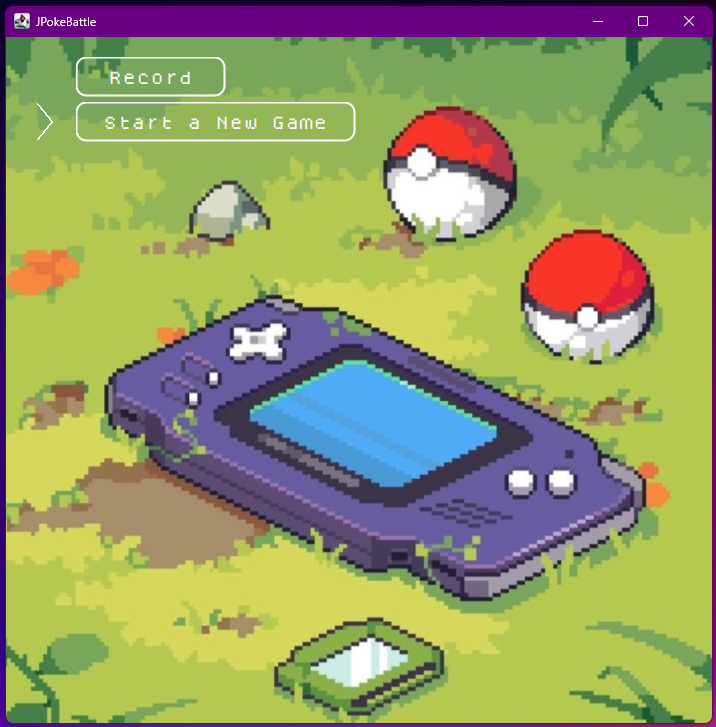
\includegraphics[width=0.45\textwidth]{Images/start.png}
    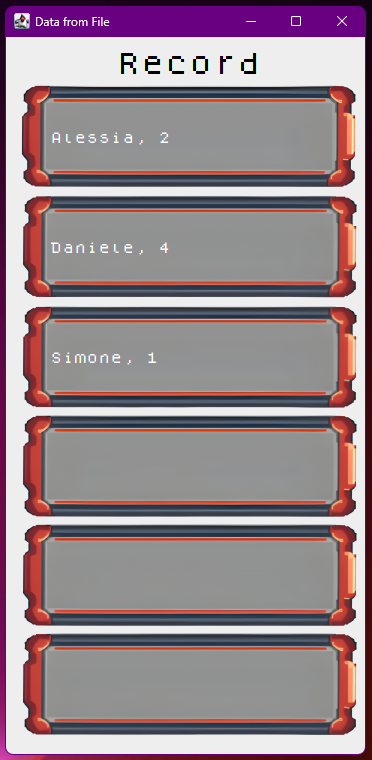
\includegraphics[width=0.22\textwidth]{Images/record.png}
\end{figure}
\newpage
\subsection{Creazione Player}
La schermata di creazione del player è la schermata in cui il giocatore può inserire il suo nome, la sua età e il suo gender.
\begin{figure}[h]
    \centering
    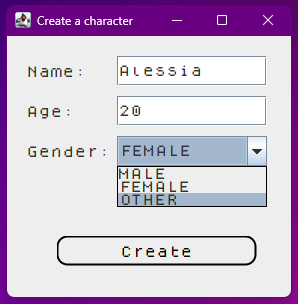
\includegraphics[width=0.35\textwidth]{Images/player.png}
\end{figure}
\subsection{Pokédex e Info Pokémon}
Il Pokèdex è una schermata in cui il giocatore può vedere i Pokémon che ha catturato. Ogni pokémon è selezionabile e permette di vedere le sue statistiche tramite un click.
Se il pokémon lo si vuole aggiungere al team si può fare tramite il bottone \textbf{Add to Team} nella schermata info. Quando il team è di gradimento del player si può cliccare sul bottone \textbf{Confirm} per andare alla battaglia successiva,
altrimenti di fianco al nome del pokemon in team c'è un pulsante che permette di rimuoverlo in caso di errore o altro.
\begin{figure}[h]
    \centering
    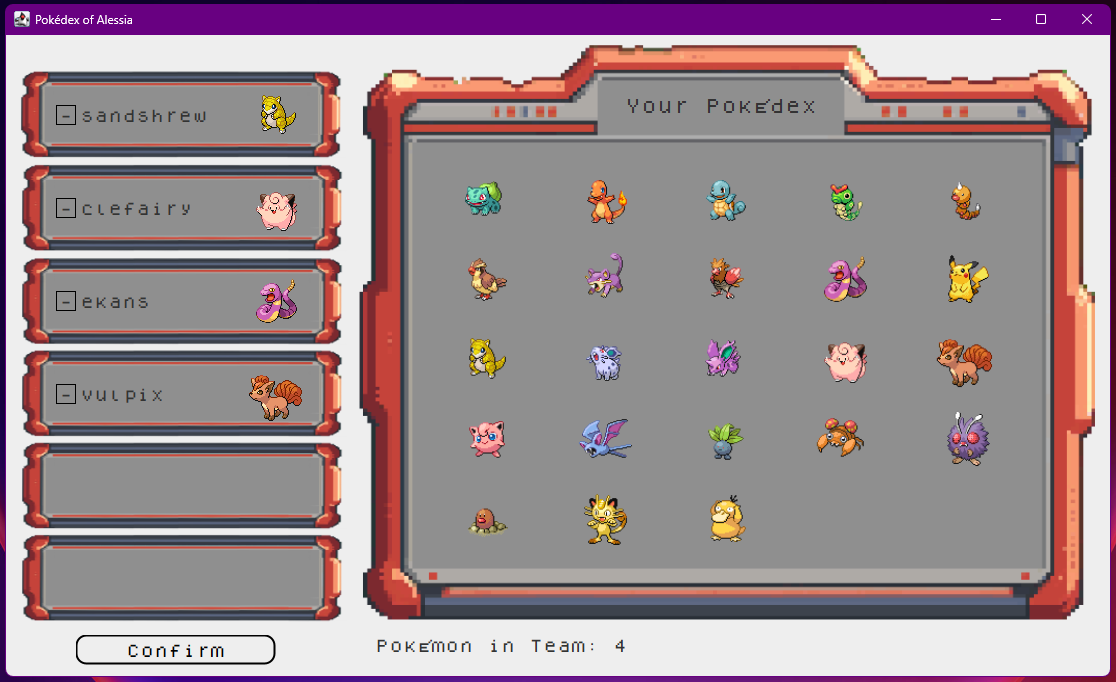
\includegraphics[width=0.55\textwidth]{Images/pokedex.png}
    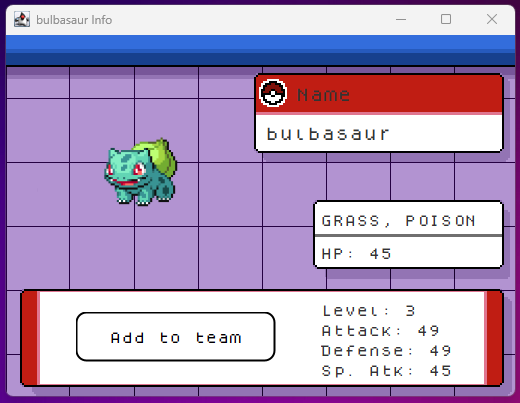
\includegraphics[width=0.44\textwidth]{Images/infopoke.png}
\end{figure}
\newpage
\subsection{Recap pre Battle}
La schermata Recap pre Battle è la schermata in cui il giocatore può vedere il team che ha scelto e in caso cambiarli.
\begin{figure}[h]
    \centering
    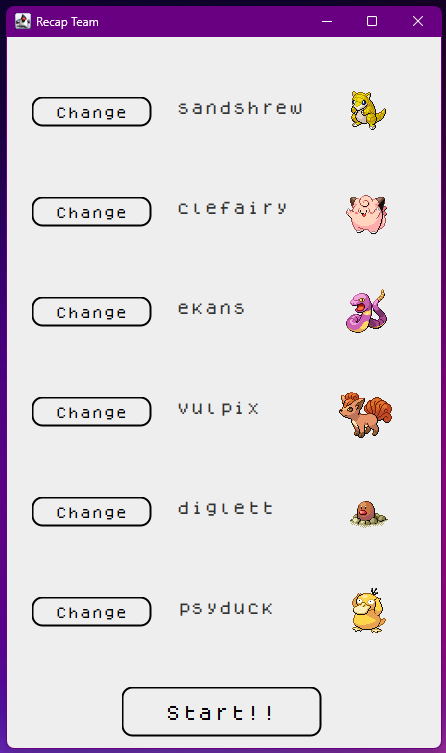
\includegraphics[width=0.25\textwidth]{Images/recapinfo.png}
\end{figure}
\subsection{Battaglia e ChangePokemon}
La schermata di battaglia è la schermata principale del gioco, in cui il giocatore può scegliere la mossa da usare o cambiare Pokémon.
Questa schermata è molto dinamica in quanto i bottoni delle mosse sono disabilitati quando non è il turno del player e viceversa, le barre degli hp diminuiscono, quella dell'exp aumenta.
Quando il pokemon del player o del nemico muore è stato sconfitto una pokéball si scurisce, questo perchè le pokéball sono indicatore di quanti pokemon ci sono nei team.
Nella schermata di Change Pokemon il giocatore può scegliere il pokémon da cambiare e il turno viene passato all'avversario, se il pokémon è in uso o stanco non è possibile selezionarlo.
\begin{figure}[h]
    \centering
    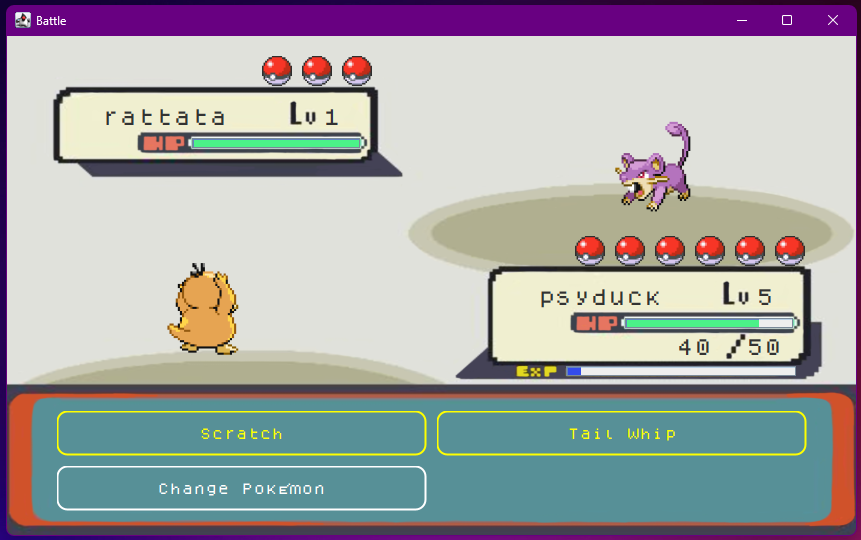
\includegraphics[width=0.55\textwidth]{Images/bsttle.png}
    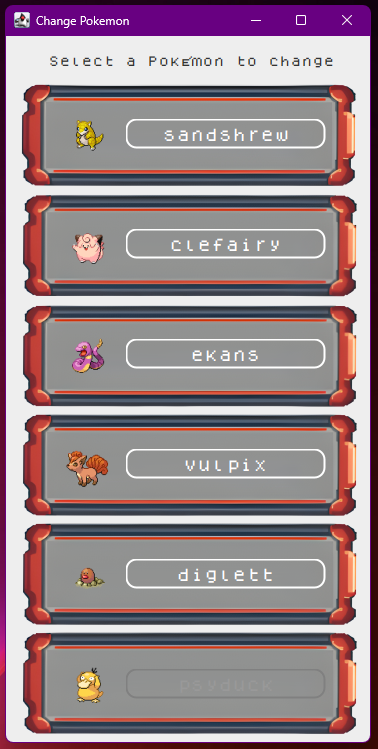
\includegraphics[width=0.20\textwidth]{Images/changepoke.png}
\end{figure}
\newpage
\subsection{RecapPost Battle}
La schermata Recap post Battle è la schermata in cui il giocatore può vedere il risultato della battaglia e le statistiche dei Pokémon in caso di vittoria.
In questa schermata il giocatore può decidere se evolvere il pokémon, cambiare una mossa o dimenticarne una per apprenderne una nuova semplicemente cliccando sui tasti appositi in caso
essi siano attivi. Se non lo sono questo implica che il pokémon non può evolversi o cambiare mossa.
\begin{figure}[h]
    \centering
    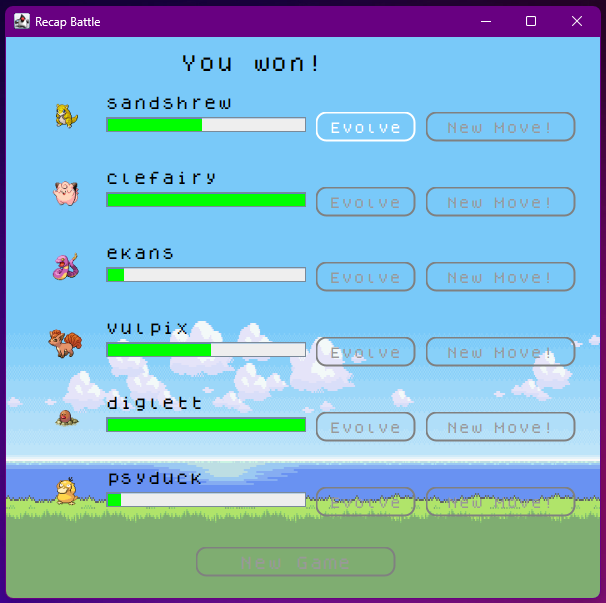
\includegraphics[width=0.45\textwidth]{Images/recapbattle.png}
\end{figure}
\subsection{Evoluzione e Change Move}
La schermata di evoluzione è la schermata in cui il giocatore può decidere se far evolvere il pokémon o meno. Una volta cliccato il bottone il frame RecapBattle si aggiornerà e mostrerà
il pokemon evoluto con gli hp del pokemon pre evoluto e le mosse aggiornate. \\ \\
La schermata di Change Move è la schermata in cui il giocatore può decidere se cambiare una mossa del pokémon con un'altra oppure no e continuare senza modiche.
\begin{figure}[h]
    \centering
    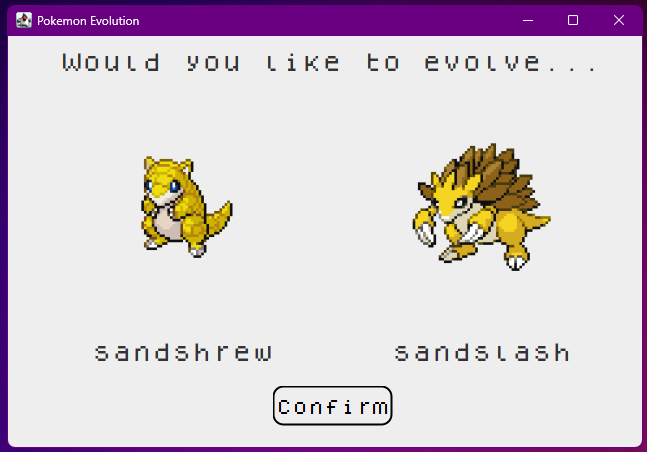
\includegraphics[width=0.35\textwidth]{Images/evolve.png}
    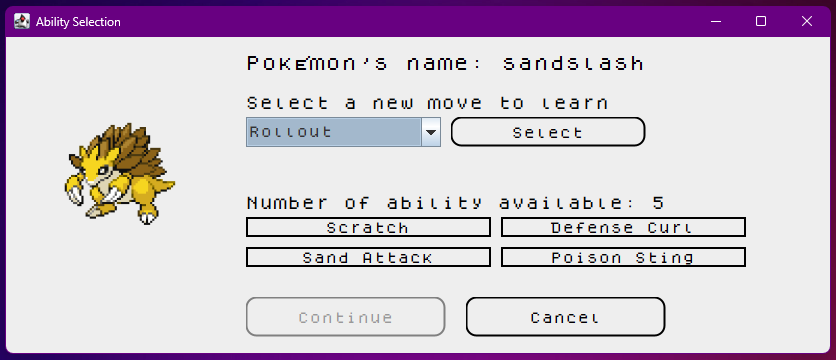
\includegraphics[width=0.55\textwidth]{Images/ability.png}
\end{figure}
\newpage
\section{Conclusioni e Ringraziamenti}
Spero che il progetto sia di gradimento e che sia stato realizzato in modo corretto. Sono soddisfatta del lavoro svolto e delle funzionalità implementate. \\ \\
Ringrazio il Professore per le lezioni svolte durante l'anno e i miei compagni di corso per l'aiuto e il supporto. \\ \\

\textbf{Alessia Cassetta}
\end{document}